\makeatletter[H]
\renewcommand{\fnum@figure}{Figure \thefigure}
\makeatother

\chapter{Experiments and Results} \label{chap:experiments}

To identify whether the Dirichlet Multinomial Regression method proposed can provide richer and more valuable information than single-output or deterministic methods can alone, we ran experiments on the data obtained from the ACFR's Sirius AUV and Schmidt's Falkor. The main machine learning algorithms' performance which we tested were Gaussian Process Classification, and Dirichlet Multinomial Regression. In this chapter, we detail the experiments designed to display the benefits of a Gaussian Process Classifier's probabilistic output, as well as the label distributions of a Dirichlet Multinomial Regressor and their respective results. \todo{(flimsy, fix)}

\section{Training Data}
To perform our experiments, bathymetry data and images of Scott Reef Central were used (the reef in the centre of \autoref{fig:scottreefaerial}). The bathymetry data was collected using Eric Schmidt's Falkor (at the locations in \autoref{fig:gridsplit}), a ship dedicated to marine research, and the (over 700GB) of images corresponding to all the bathymetry data was collected by The University of Sydney's Australian Centre for Field Robotic's Sirius Autonomous Underwater Vehicle (AUV). The training set provided already had labels assigned, which was a result of previous efforts using Variational Dirichlet Processes that performed the unsupervised clustering \citep{steinberg11}. On close inspection, the UTM coordinates in the training set do not correspond to the original data available from \cite{squidle} - this was because the exact point of retrieval for the bathymetry and image weren't exact matches. To account for this, labels corresponding to bathymetry points were in fact taken from the closest images, rather than exact longitude/latitude or UTM matches, although the UTM coordinates in the training data itself remains as the original.

\todo{(describe the specific features - depth, aspect, rugosity, etc.)}

\begin{figure}
    \includegraphics{scott_reef_aerial.jpg}
    \caption{Aerial shot of Scott Reef from \cite{NASA:SRI}}
    \label{fig:scottreefaerial}
\end{figure}

\section{Data Preprocessing}

\subsection{Downsampling the Data}
As the purpose of using Dirichlet Multinomial Regression was to be able to model the distribution of habitat label occurrences over an area, we downsampled the combined 2011+2015 dataset which was at a siginficantly higher resolution than the 2009 dataset \todo{(calculate how much perhaps)}. Two methods of downsampling in particular were tested. The first coarser approach involved simply taking the space in which the data was collected and placing grids of fixed size over them as in \cref{fig:gridsplit}, binning all points falling within each grid into a single datapoint. Each of these data points contained multiple points from the original dataset with their own counts for each of the possible labels, so the downsampled points simply took the sum of all the label counts in each fixed grid. 

The second summed label counts in the same way, but clusters were instead formed by first calculating the full dendrogram on the 16502 entries in the training data, and forming groups such that none had more than 5 of the original points within them, and the sub-clusters (at each level of the dendrogram) were no more than a 21 metres away from one another. As can be seen in \cref{fig:dendrogram}, the gradual merging into the single supercluster was quite consistent, indicating the original datapoints were mostly evenly distributed.

For a fair comparison between Gaussian process classification and dirichlet multinomial regression, the downsampled data was used to train the GPs as well - although this seems like an unnecessary handicap to the GP, it is more appropriate considering that one of the aims here is to demonstrate what sort of information can be gained from a DM vs. a GP, given the same \textit{raw} data.

\todo{(cut down this section (probably down to one paragraph) - and also talk about how for the single label case, instead of summing counts for the new 'label', labels were chosen at random (for more variance in the GP which is otherwise too certain about everything being sand))}

\begin{figure}[H]
    \includegraphics[scale=0.6]{training_map_fixedgrid.pdf}
    \caption{Fixed-sized grids placed over training data}
    \label{fig:gridsplit}
\end{figure} 
\begin{figure}[H]
    \centering
    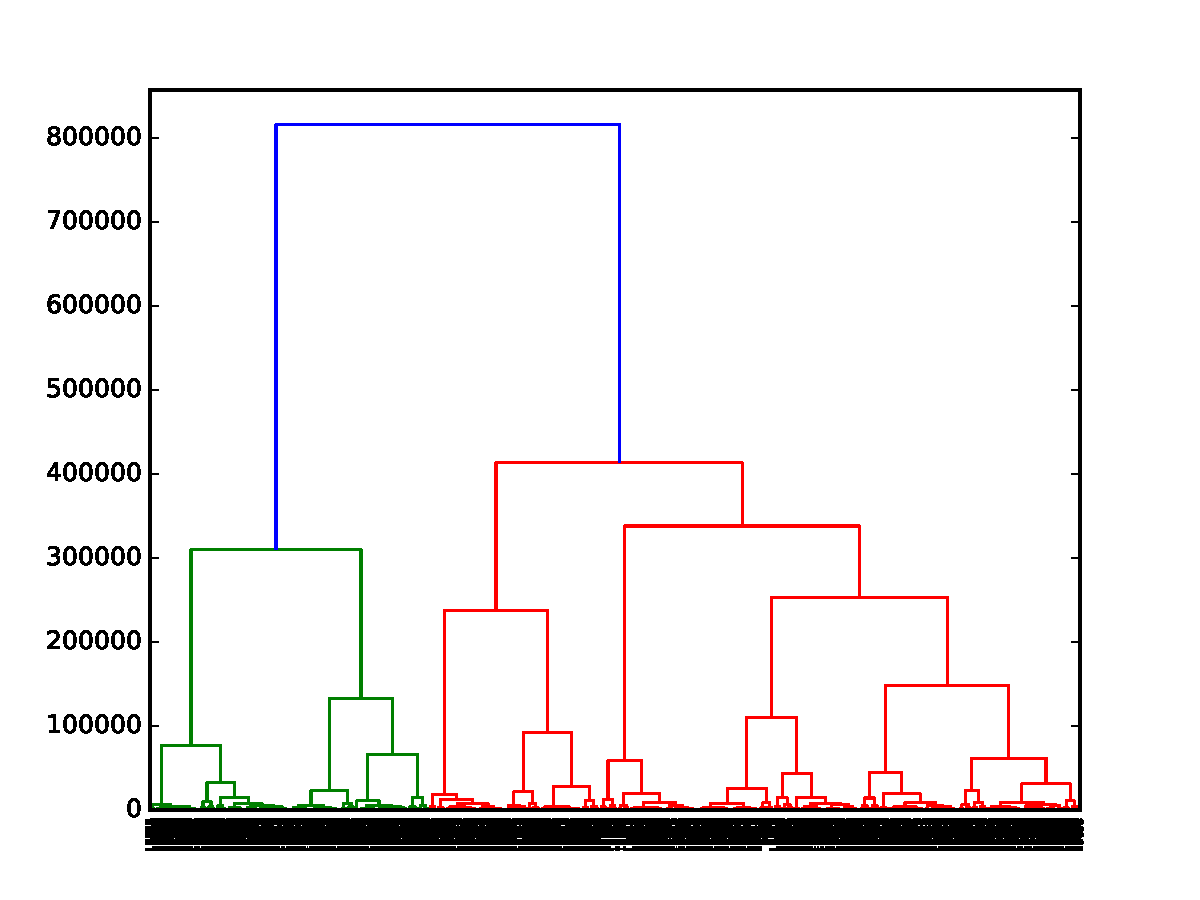
\includegraphics[scale=0.6]{dendrogram.pdf}
    \caption{Dendrogram of training data}
    \label{fig:dendrogram}
\end{figure}

\subsection{Simplifying labels}
Another step that was considered during experiments was the aggregation of habitat labels. The original training data contained 24 separate labels determined through an automated clustering procedure using Dirichlet Processes. Because of the uneven distribution of these labels (\autoref{fig:singlelabeldistr} and \autoref{fig:multilabeldistr}), with the occurrence of some too insignificant for any machine learning algorithms to pick up, they were simplified in collaboration with ecological experts, who manually identified which of the 24 labels were in fact of the same class - for example, 5 separate classes of coral may have been indistinguishable to the average person, and were hence grouped into a single label. This allowed the near-non-occurring labels to be grouped together with more commonly occurring ones, whilst also allowing a different level of granularity in training models/forming predictions that could be used if only an approximation equivalent to observable human differences of an area's benthic map were required. Moreover, due to the unsupervised nature of the labeling, certain clusters were notably \textit{inconsistent} with the rest, for example when sea cucumbers became the identifying feature of one of the 24 labels.

\begin{table}[H]
    \centering
    \begin{tabular}{|c| c|}
        \hline
        simplified & original \\\hline
        0 & 1, 2, 18, 20, 21, 23, 24 \\
        1 & 3, 5, 10, 16, 17, 19, 22\\
        2 & 13, 14, 15 \\
        3 - Sand & 4, 6, 7, 8, 9, 11, 12 \\
        \hline
    \end{tabular}
    \caption{Full-simplified label mappings \tiny{\todo{label mappings - sand, coral, patchy coral, (?) halameda, rhodliths}}}
    \label{table:labelmappings}
\end{table}

\begin{figure}
    \includegraphics[scale=0.17]{class_mosaic_24_classes.jpg}
    \caption{Samples of images from each of the full 24 classes}
    \label{fig:24classes}
\end{figure}

\begin{figure}[H]
    \begin{minipage}{.47\linewidth}
        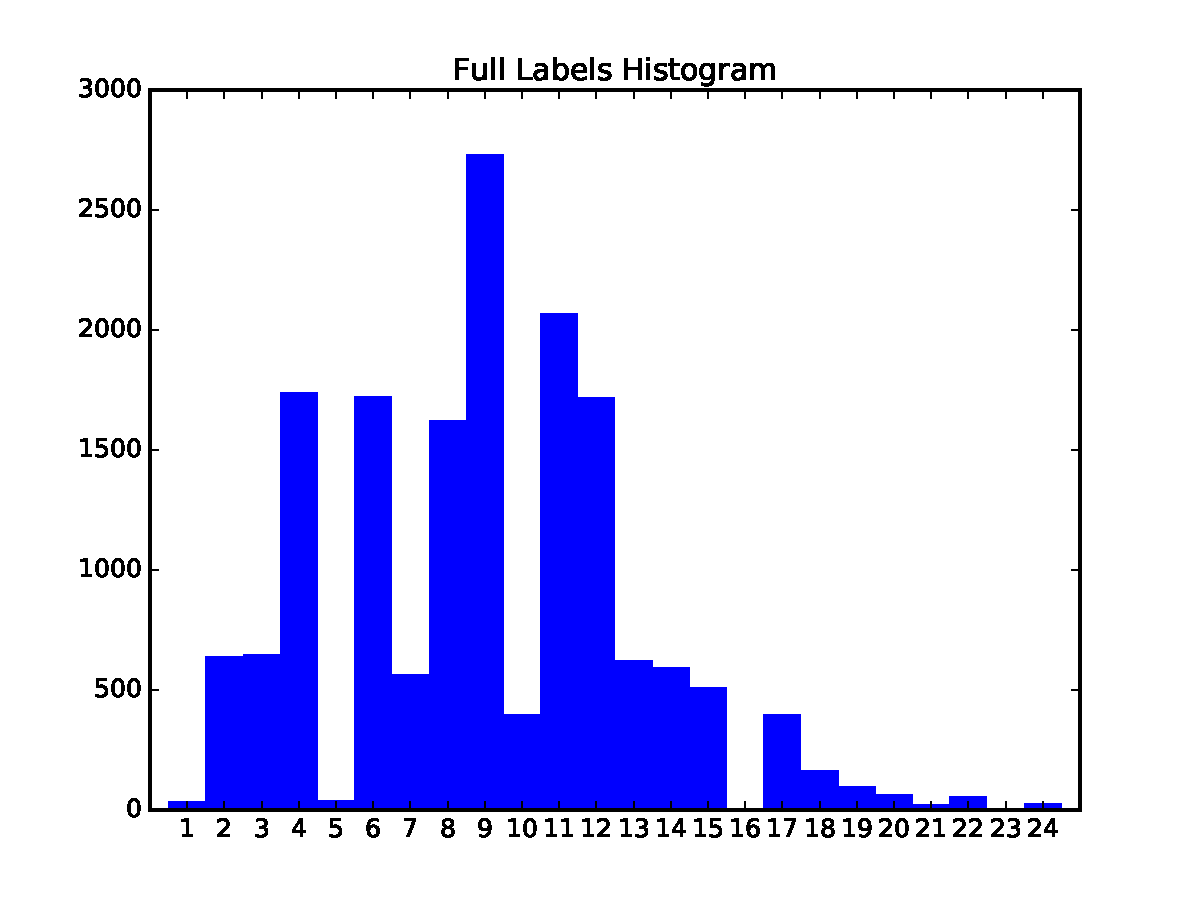
\includegraphics[width=\linewidth]{hist_full_labels.pdf}
        \caption{Distribution of labels in original dataset}
        \label{fig:singlelabeldistr}
    \end{minipage}
    \hfill
    \begin{minipage}{.47\linewidth}
        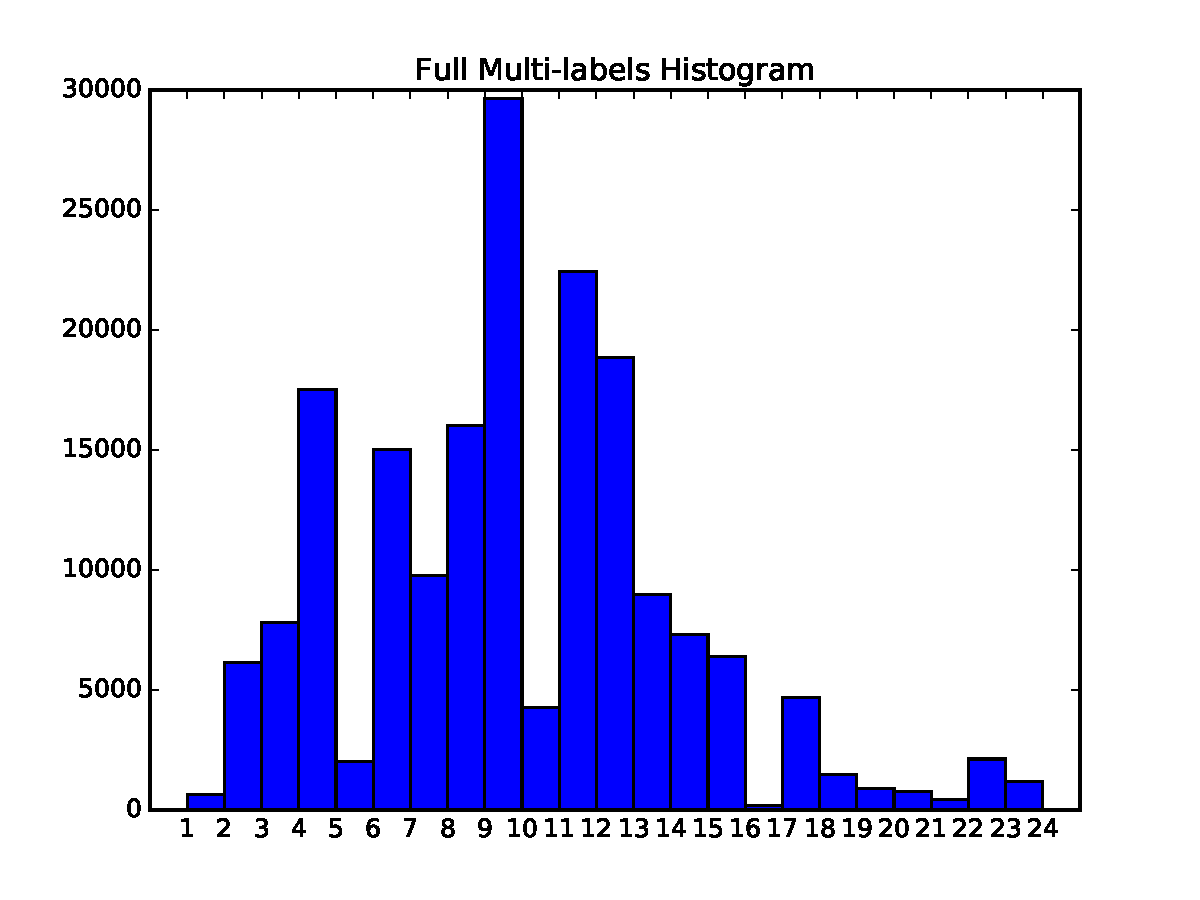
\includegraphics[width=\linewidth]{hist_full_multi_labels.pdf}
        \caption{Distribution of labels in multi-label outputs}
        \label{fig:multilabeldistr}
    \end{minipage}
\end{figure}

\begin{figure}[H]
    \begin{minipage}{.47\linewidth}
        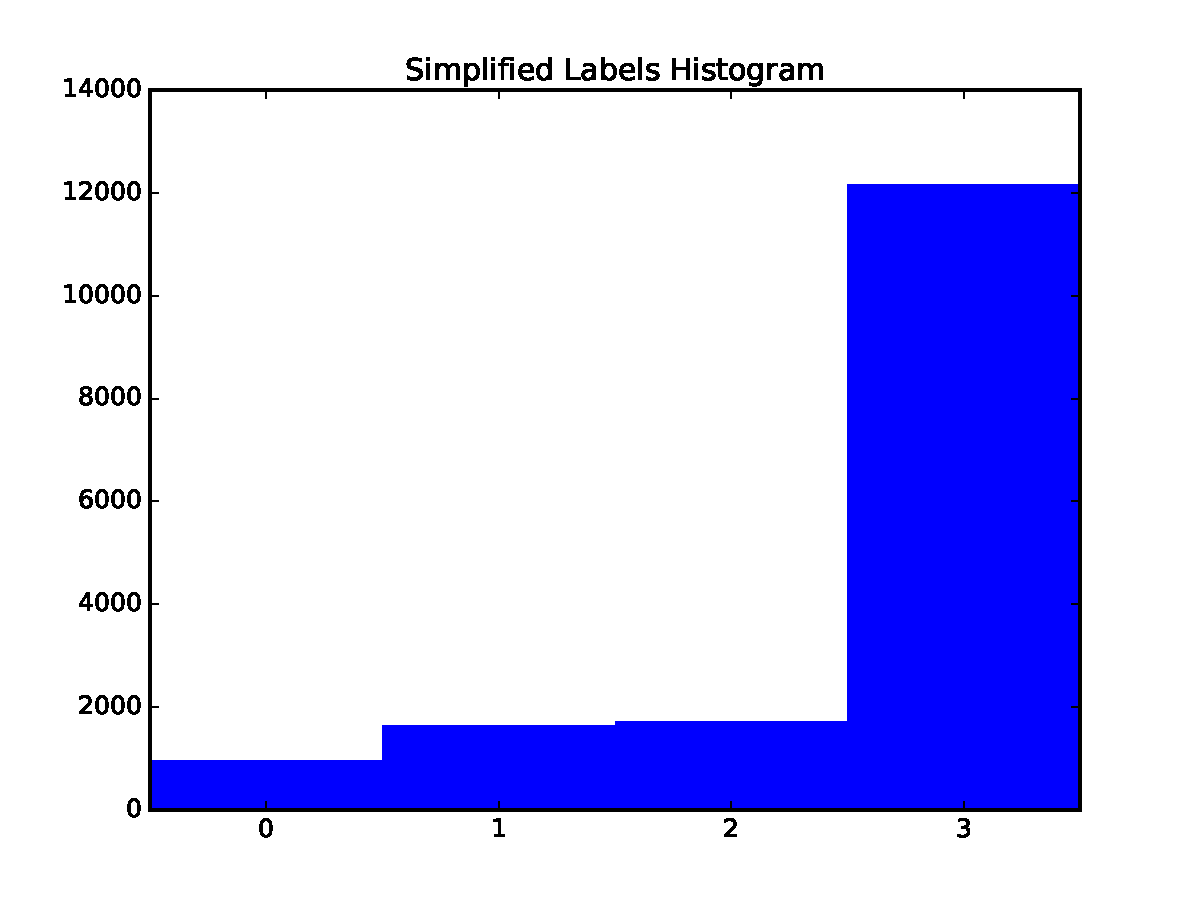
\includegraphics[width=\linewidth]{hist_simple_labels.pdf}
        \caption{Distribution of simplified labels in original dataset}
        \label{fig:singlelabeldistr}
    \end{minipage}
    \hfill
    \begin{minipage}{.47\linewidth}
        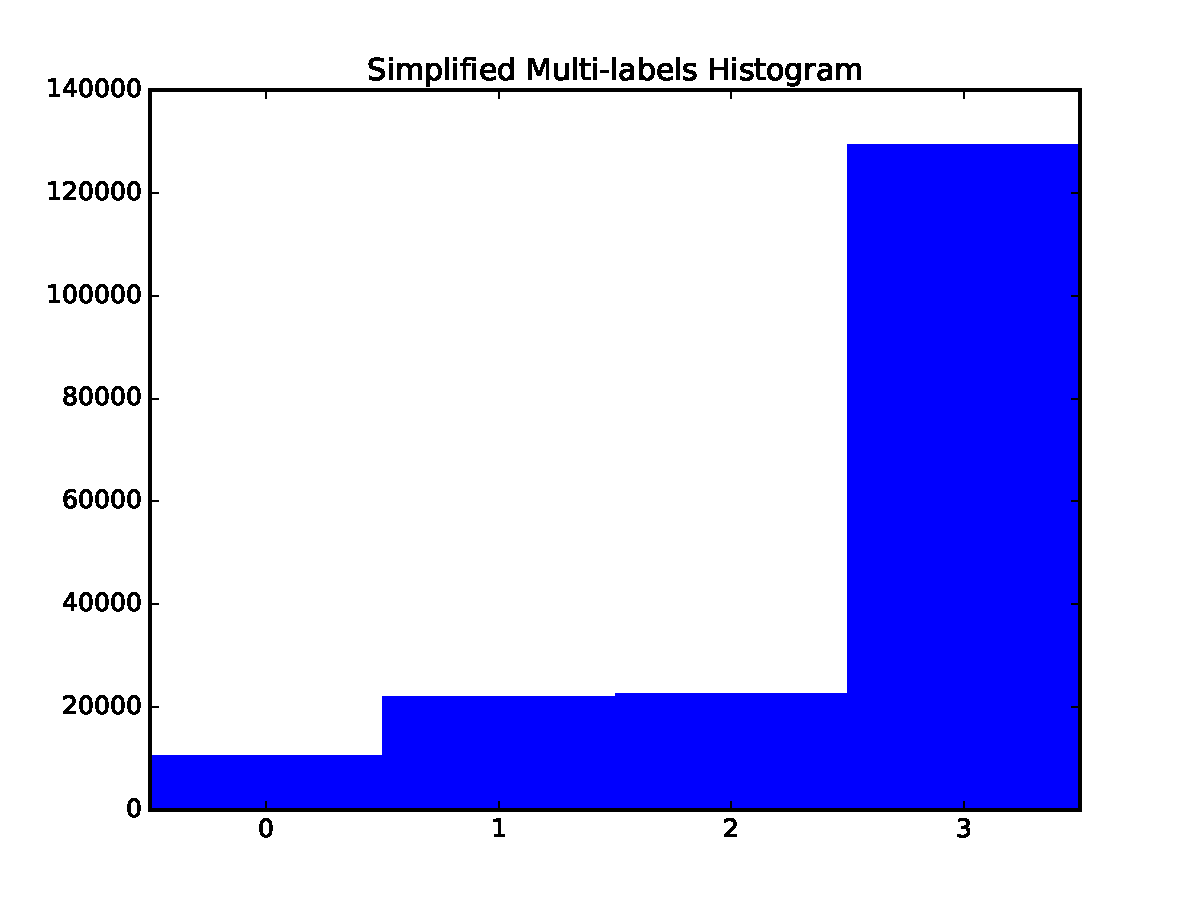
\includegraphics[width=\linewidth]{hist_simple_multi_labels.pdf}
        \caption{Distribution of simplified labels in multi-label outputs}
        \label{fig:multilabeldistr}
    \end{minipage}
\end{figure}

Note that from this point onwards, we will be working with the reduced feature set, in line with the aim of the paper to show the advantages of dirichlet multinomial regression when studies (environmental or otherwise) are limited to lower resolution data where strictly assigning only a single label to the features at a given data point is not representative of the otherwise rich information available.

\subsection{Coordinates as features}
Due to the abundant bathymetry data that was available in the form of depth, rugosity and aspect at each available data point, there was reason not to include the coordinates themselves in the feature space. Whilst it does make sense that in a natural environment, areas that were spatially near to one another would also have similar properties, this should not be relied upon, and other intrinsic properties should be the basis upon which predictions are made. Forming predictions on the full query dataset using a random forest supports this notion quite strongly - whilst 10-fold cross validation using the coordinates as features had a notably higher F-score of 0.61 compared to 0.40 without, the unnaturally straight split between the left and right segments over a 12km region suggests that the predictive map is flawed. Moreover, by including the coordinates as a training feature, an assertion is made about the direct relationship between a benthic location and the habitat class/es it contains, despite having other bathymetry information such as depth, aspect, etc. 

\todo{(argument/s here alone is/are weak. for simplified labels using coords is still much better by a similar (small) margin, do some reading to back this up properly)}

\begin{figure}[H]
    \begin{minipage}{.49\linewidth}
        \includegraphics[width=\linewidth]{full_predictions_randomforest.pdf}
        \caption{Full predictive map using Random Forests including coordinates as features}
        \label{fig:rf_w_coords_preds}
    \end{minipage}
    \hfill
    \begin{minipage}{.49\linewidth}
        \includegraphics[width=\linewidth]{full_predictions_randomforest_nocoords.pdf}
        \caption{Full predictive map using Random Forests excluding coordinates as features}
        \label{fig:rf_wo_coords_preds}
    \end{minipage}
\end{figure}

\subsection{Preprocessing and Feature Projection}
To maximise performance (in terms of minimising error/maximising the correctness metrics used) of the algorithms used across the experiments, a number of preprocessing steps were taken to ultimately improve the performance of the predictions made. The features in the data were first scaled, where each feature was centred to the mean with unit variance), then normalised over each future such that they had unit length \todo{(include plots of the diff approaches across DM/GP/others, ref plots)}. To further minimise bias and variance\todo{(maybe add to this technically)}, the original feature set (which from this point onwards refers to all the non-coordinate features) was projected into degree-2 space with a $1$-bias term. For example, given features $x_0, x_1, x_2, x_3$ is projected to $1, x_0, x_1, x_2, x_3, x_0^2, x_1^2, x_2,^2, x_3^2$. This projection was chosen from comparing the performance of different projections

\todo{(ref plots)}

\todo{(show plots)}

As evident from above, adding the square ($^2$) of each feature with a 1 regulariser \todo{(figure out what 1 column should be called)} yielded in performance that was negligibly lower ($\sim 1e-5$) than projection into full quadratic space, whilst requiring considerably fewer features - 19 for the former, vs. 55 for the latter. While this difference isn't significant for GPs \todo{(perhaps provide a time benchmark for this too)}, it has a significant effect on running time later on when using Markov Chain Monte Carlo (MCMC) to obtain draws of the weights of the Dirichlet Multinomial Regressor - when working with the simplified 4-label case, there are $19*4 =76 \text{ vs. } 55*4=220$ weights, i.e. dimensions to deal with, whereas the full 24-label case would involve $19*24=456$ and $55*24=1320$ weights respectively, which would result in a very significant increase in computing power needed for the MCMC chains to converge in the latter case, relatively speaking.

The results from the Experiments detailed in Chapter 4 are listed below. The range of possible class values in some cases have been stretched beyond the existing class labels so that values align between different outputs to allow for easy, direct visual comparison \todo{(this hasn't actually happened yet)}. Note that the results to the above experiments will include those of both non-downsampled and downsampled results, as well as the full set of 24 labels as well as simplified ones.

Due to the low occurrence of some labels in the original dataset though, they have ended up being ommitted in predictions - these are excluded from the colour schemes of the benthic maps generated, so that those that do occur can be given more distinct colours from one another as to better differentiate between the habitats of a map, as well as allow a consistent comparison of across different maps. \todo{(again, hasn't happened yet)}

% The associated generated maps from the experiments are also provided here, but proper evaluation of them, such as what habitat clusters and relationships can be gleaned, will be explored in Chapter 5. 

\pagebreak
\section{Deterministic Methods}

To first set a baseline for predictions over the bathymetry dataset, we look at the performance of some deterministic methods with respect to their unweighted (average of each label) f-scores. Logistic regression has been included here despite containing 'probabilistic` predictions in the form of regression values passed through the \textit{logit}, and as such the results displayed are a result of simply taking the argmax over possible the predictive probability over possible for each datapoint. Those probabilistic outputs are useful for comparisons with those of Gaussian Processes, however, which will be explored in the next section. \todo{(hasn't happened yet)}

\begin{table}[H]
    \centering
\begin{tabular}{|c|c|c|c|c|c|}
    \hline
    Algorithm & 10F-CV F1 & 10F-CV Accuracy & Label type\\\hline
    SVC & 0.21514 & 0.75554 & 4 labels \\
    LogisticRegression & 0.33713 & 0.77001 & 4 labels \\
    KNeighborsClassifier & 0.4714 & 0.7796 & 4 labels \\
    RandomForestClassifier & 0.4737 & 0.79406 & 4 labels \\
    SVC & 0.10355 & 0.29408 & 24 labels \\
    LogisticRegression & 0.13335 & 0.31389 & 24 labels \\
    KNeighborsClassifier & 0.22593 & 0.33093 & 24 labels \\
    RandomForestClassifier & 0.22015 & 0.3405 & 24 labels \\
    \hline
\end{tabular}
\label{table:detresults}
    \caption{Performance of common machine learning models}
\end{table}

While the accuracy of the Logistic Regressor, kNN, and Random Forest Classifier are reasonable (above $0.75$), the former two's f1-scores are very poor at $0.33$, with the latter two at just below $0.5$, which is an equally undesirable result. Looking at the ratio of available labels in the downsampled data in the 4-label case ($232,  470,  446, 3548$ for labels 0, 1, 2, 3 respectively) reveals that label 3 accounts for $0.7556$ of the dataset - a value very close to the accuracy of predict. the weighted f1-score of a `naive' classifier that always predicts label 3 has an accuracy of  $0.75554$ and weighted f1 score of $0.6503$ - highlighting the fact that these simpler models are not able to produce results that confidently outperform simply guessing one label for any given datapoint. \autoref{fig:det4maps} below shows the predictions of each of the above predictions on the full query data for the 4 and 24-label data respectively.

\begin{figure}[H]
    \includegraphics[width=\linewidth]{det_preds.pdf}
    \caption{Full predictive map using Random Forests excluding coordinates as features}
    \label{fig:det4maps}
\end{figure}

\section{Gaussian Process Classification}

\todo{transfer all the results from markdown}

\todo{show more stratified results (not just even split) to show that even splits did better}

\begin{tabular}{|c|c|c|c|c|c|c|c|}
    \hline
    No. points & Type of split & Type of GP & Number of runs & AUROC & Notes & F1-score \\\hline
    500     & Even       & GP     &  10        & 0.86534    &                     &         \\
    500     & Stratified & GP     &  10        & 0.80136    &                     &         \\
    1000    & Even       & GP     &  1         & 0.87626    & Deterministic       & 0.56208 \\
    1000    & Even       & PoEGP  &  5         & 0.80973    &                     & 0.47481 \\
    1000    & Even       & PoEGP  &  200       & 0.80186    &                     & 0.47595 \\
    1000    & Even       & GPoEGP &  5         & 0.80864    &                     & 0.51018 \\
    1000    & Even       & GPoEGP &  200       & 0.80105    &                     & 0.47748 \\
    1000    & Even       & BCM    &  5         & 0.80682    &                     & 0.48167 \\
    1000    & Even       & BCM    &  200       & 0.80421    &                     & 0.48227 \\
    1000    & Even       & GPy    &  1         & 0.87638    & RBF, EP (default)   & 0.57013 \\
    \hline
\end{tabular}
\todo{(look at AUROC/AUC and log probabilities as well)}

\todo{highlight areas with low/high certainty, etc. NOTE - investigate the areas with visually even splits of two labels - e.g. right-side arms of label 1,2, and smaller patches in the bottom left corner of label 0,3 - show that uncertainty about whether those areas are label 1 or 2, 0 or 3 respectively, is (should) be high, and that taking argmax for the sake of visual representation within a single image hides this information}

\todo{(maps of 4-label full predictions)}

\todo{(maps of all-label full predictions)}

\subsection{Using Multiple Gaussian Process Regressors per normalised Multi-output label}
Average error was $0.14409166865082482$ in 10-fold CV


\section{Dirichlet Multinomial Regression}

% \begin{tabular}{|c|c|c|c|c|c|}
%     \hline
%     Algorithm & 10F-CV F1 & 10F-CV Accuracy & Parameters & Data \\\hline
%          DM         &  0.13802716811804644 & 0.37856057852908254 &            &  full labels  \\
%          DM         &   0.287405310254214  &  0.757925654489819  &            & simple labels \\ %     \hline
% \end{tabular}

\subsection{Parameter Selection}

To select an optimal set of parameters for the dirichlet multinomial, Markov Chain Monte Carlo (MCMC) was used to draw samples from the posterior distribution \todo{(refer to equation?)} over $3,000,000$ runs, with the maximum a posteriori estimate used as the starting value for the weights. To select the single best set of weights from the sequence of chains, every single one was evaluated by being used to do Dirichlet Multinomial regression, where the weights that resulted in the lowest predictive variance (average over all variances) was considered to be the best set of parameters. The weights that corresponded to the lowest average variance also corresponded to the lowest average error compared to the original normalised weights. After the $3,000,000$ runs, the MCMC in both cases (the simplified 24 labels, as well as the full set) was considered to have converged, as the Gelman and Rubin ($\hat{r}$) convergence statistics were calculated to be \todo{(? and ?)}, both very close to the ideal value of $1.0$, Furthermore, for the \todo{24-label case}

% MCMC 2 million runs, 24 labels
% 18-smallest variance corresponds to the 1-smallest error - index 1444288 \\
% 19-smallest variance corresponds to the 2-smallest error - index 1444289 \\
% 20-smallest variance corresponds to the 4-smallest error - index 1444292 \\
% 21-smallest variance corresponds to the 0-smallest error - index 1444291 \\
% 22-smallest variance corresponds to the 3-smallest error - index 1444290 \\

% np.save('data/W_2m_1444288', chains[1444288])
% np.save('data/W_2m_1444289', chains[1444289])
% np.save('data/W_2m_1444292', chains[1444292])
% np.save('data/W_2m_1444291', chains[1444291])
% np.save('data/W_2m_1444290', chains[1444290])

\begin{figure}[H]
    \centerline{\includegraphics{dm4_9m_0_mcmc_weight_hist.pdf}}
    \caption{MCMC weights for 4-label, 19-dimension data case \todo{(need to separate this into separate images, possibly remove axis ticks)}}
    \label{fig:4l-mcmc_weights}
\end{figure}

\begin{figure}[H]
    \centerline{\includegraphics{dm24_950k_0_mcmc_weight_hist.pdf}}
    \caption{MCMC weights for 4-label, 19-dimension data case \todo{(need to separate this into separate images, possibly remove axis ticks)}}
    \label{fig:24l-mcmc_weights}
\end{figure}

\begin{table}[H]
    \centering
    \begin{tabular}{|c|c|}
        \hline
        Features & Root Mean Squared Error \\\hline
        Original features, using coordinates & 0.3360700584111156 \\
        Original features, not using coordinates & 0.33676707345298545 \\
        Quadratic projection, using coordinates & 0.19695170465540882 \\
        Quadratic projection, not using coordinates & 0.19726479764111976 \\
        \hline
    \end{tabular}
    \label{table:dmbasicresults}
    \caption{Dirichlet Multinomial Regression results}
\end{table}

In line with what was observed in the DM illustrative example in \autoref{table:toy_gm_vs_gp}, performance was better when taking the quadratic projection of the original features - though in this case, the improvement was much more significant, namely by 41.4\% compared to the 6.5\% in the illustrative example. \todo{(numbers here will change})

As a means of effectively visuailsing the separate labels, we need to look at the normalised distribution of habitat classes for each label separately. This allows initial observations to be made of where certain labels are more abundant than others. Immediately, we can see the concrete advantages of using a multi-output model, as individual points no longer contain only a single label - \autoref{fig:dm_4label_heatmap} for example, shows that the majority of the reef is predominantly sand (label 3) with smaller proportions of the other labels, with the bottom-left region being mostly an even combination of labels 1, 2 \todo{(get actual labels)} and scattered sections of sand. Using the approaches previously explored, it would not have been directly inferable (without extra processing of labels/results) that the sand-dominant areas also contained small amounts of other labels.

% that the outreaching \textit{arm-like} portions on the right hand side of Scott Reef Central contain large areas of even splits of label 1 and 2, with trace amounts of label 0, but almost no label 3, which is otherwise the most frequently occuring habitat in the area \todo{(get the \textbf{actual} label names!)}.

\begin{figure}[H]
    \begin{minipage}{\linewidth}
        \centerline{\includegraphics{dm_standalone_colorbar.pdf}}
        \centerline{\includegraphics{dm_simplelabel_heatmaps.pdf}}
        \caption{Distribution heatmaps over each label (in the simple 4-label case) for Dirichlet Multinomial Regressor output on query points}
        \label{fig:dm_4label_heatmap}
    \end{minipage}
    \hfill
\end{figure}

In contrast to the GP above where the uncertainty was greatest when there were even distributions of labels, it is expected that the DM would be comparitively more confident that an even mix of labels exist in these areas. To obtain a sufficiently large area/number of points where two of the simplified four labels had a fairly even occurrence rate (with the other two labels only having trace amounts, if at all), pairs of labels were repeatedly sampled with the variable condition that both their distributions lie within a certain range (for example, $[0.4, 0.5]$, or $[0.2, 0.3]$), until a segment was found where the average variance over these points were significantly lower than the variance in label distributions across the overall predictions. The variance in this regions were then compared to that of a Gaussian Processes'.

\todo{summarise and plot the variances here}

What becomes apparent is that in the areas where the DM is confident of a mix of certain set of predominant labels, the GP is instead equally uncertain of each of them with a considerably higher variance, which is misleading information when taken at face value. For example, this sort of uncertainty may be taken into consideration purposes, where autonomous vehicles are used to collect data, or in making decisions with regards to conservation efforts. In the first scenario, resources are being wasted on areas where models such as the DM can be confident of a particular distribution of labels, whereas in the second, important conservation actions may be withheld if the \textit{certainty} of information is brought into question. For example, in an area that contains a particular mix of coral and bleached coral, a DM has the potential to make a confident prediction of their coexistence, whereas a GP would make predictions where their respective probabilities in a one-vs-all classifier may be close to their distribution in the area, but have a high noise factor.

\begin{figure}[H]
    \textbf{DM Full Label 1-6 Predictions}
    \centerline{\includegraphics[scale=0.85]{dm_standalone_colorbar.pdf}}
    \centerline{\includegraphics[scale=1.0]{dm_alllabels_heatmap_1-6.pdf}}
    \caption{Distribution heatmaps over labels 1-6 (in the full 24-label case) for Dirichlet Multinomial Regressor output on query points}
    \label{fig:dm_24-1_label_heatmap}
    \hfill
\end{figure}
\begin{figure}[H]
    \textbf{DM Full Label 7-12 Predictions}
    \centerline{\includegraphics[scale=0.85]{dm_standalone_colorbar.pdf}}
    \centerline{\includegraphics{dm_alllabels_heatmap_7-12.pdf}}
    \caption{Distribution heatmaps over labels 7-12 (in the full 24-label case) for Dirichlet Multinomial Regressor output on query points}
    \label{fig:dm_24-2_label_heatmap}
    \hfill
\end{figure}
\begin{figure}[H]
    \textbf{DM Full Label 13-18 Predictions}
    \centerline{\includegraphics[scale=0.85]{dm_standalone_colorbar.pdf}}
    \centerline{\includegraphics{dm_alllabels_heatmap_13-18.pdf}}
    \caption{Distribution heatmaps over labels 13-18 (in the full 24-label case) for Dirichlet Multinomial Regressor output on query points}
    \label{fig:dm_24-3_label_heatmap}
    \hfill
\end{figure}
\begin{figure}[H]
    \textbf{DM Full Label 19-24 Predictions}
    \centerline{\includegraphics[scale=0.85]{dm_standalone_colorbar.pdf}}
    \centerline{\includegraphics{dm_alllabels_heatmap_19-24.pdf}}
    \caption{Distribution heatmaps over labels 19-24 (in the full 24-label case) for Dirichlet Multinomial Regressor output on query points}
    \label{fig:dm_24-4_label_heatmap}
    \hfill
\end{figure}

\subsection{Biodiversity}
\todo{highlight areas with biodiversity, particular co-occurring species, etc.}

Another beneficial aspect of DMs are that they can inherently provide information about the distribution of different habitats in a given region, allowing observations on biodiversity to be made without requiring extra post-processing steps such as clustering, which can be prohibitively expensive on datasets with millions of datapoints and tens (or more) of dimensions. To locate certain co-existence of species, the only step required would be to search over the space of predictions for the desired distributions simultaneously, assigning each a particular portion, with a margin of error. For example, we could easily locate areas with mixes of \todo{(change here for a good example)} labels 5, 9, and 14, with each having an even split with a margin of $0.05$ - this would result in us searching the predictions with the conditions where label 5 has a predictive distribution $[0.28, 0.38]$, as would labels, 9, 14. 

\todo{(some plots of these - pick ones that have `nice' graphs)}

The above scenario assumes, however, that an ecologist (or anyone using the data) is already aware of the proportions of habitats they are searching for, which may not be the case if \todo{(describe a scenario here where the application is to detect changes in biodiversity over time)}
